% Created 2020-03-12 Thu 13:17
% Intended LaTeX compiler: pdflatex
\documentclass[a4paper]{article}

\usepackage{booktabs}
\usepackage[margin=2cm]{geometry}
\usepackage{sourcecodepro}
\usepackage{booktabs}
\usepackage{array}
\usepackage{colortbl}
\usepackage{listings}
\usepackage{algpseudocode}
\usepackage{algorithm}
\usepackage{graphicx}
\usepackage[english]{babel}
\usepackage[scale=2]{ccicons}
\usepackage{hyperref}
\usepackage{relsize}
\usepackage{amsmath}
\usepackage{bm}
\usepackage{amsfonts}
\usepackage{wasysym}
\usepackage{float}
\usepackage{ragged2e}
\usepackage{textcomp}
\usepackage{pgfplots}
\usepackage{todonotes}
\usepgfplotslibrary{dateplot}
\lstdefinelanguage{Julia}%
{morekeywords={abstract,struct,break,case,catch,const,continue,do,else,elseif,%
end,export,false,for,function,immutable,mutable,using,import,importall,if,in,%
macro,module,quote,return,switch,true,try,catch,type,typealias,%
while,<:,+,-,::,/},%
sensitive=true,%
alsoother={$},%
morecomment=[l]\#,%
morecomment=[n]{\#=}{=\#},%
morestring=[s]{"}{"},%
morestring=[m]{'}{'},%
}[keywords,comments,strings]%
\lstset{ %
backgroundcolor={},
basicstyle=\ttfamily\scriptsize,
breakatwhitespace=true,
breaklines=true,
captionpos=n,
extendedchars=true,
frame=n,
language=R,
rulecolor=\color{black},
showspaces=false,
showstringspaces=false,
showtabs=false,
stepnumber=2,
stringstyle=\color{gray},
tabsize=2,
}
\renewcommand*{\UrlFont}{\ttfamily\smaller\relax}
\author{Pedro Bruel}
\date{\today}
\title{Weighted Sum of Averages of Injection Rates and Execution Times}
\hypersetup{
 pdfauthor={Pedro Bruel},
 pdftitle={Weighted Sum of Averages of Injection Rates and Execution Times},
 pdfkeywords={},
 pdfsubject={},
 pdfcreator={Emacs 26.3 (Org mode 9.2.5)},
 pdflang={English}}
\begin{document}

\maketitle
The figure  below shows the injection  rates, for both applications,  in the 200
samples tested.

\begin{figure}[htbp]
\centering
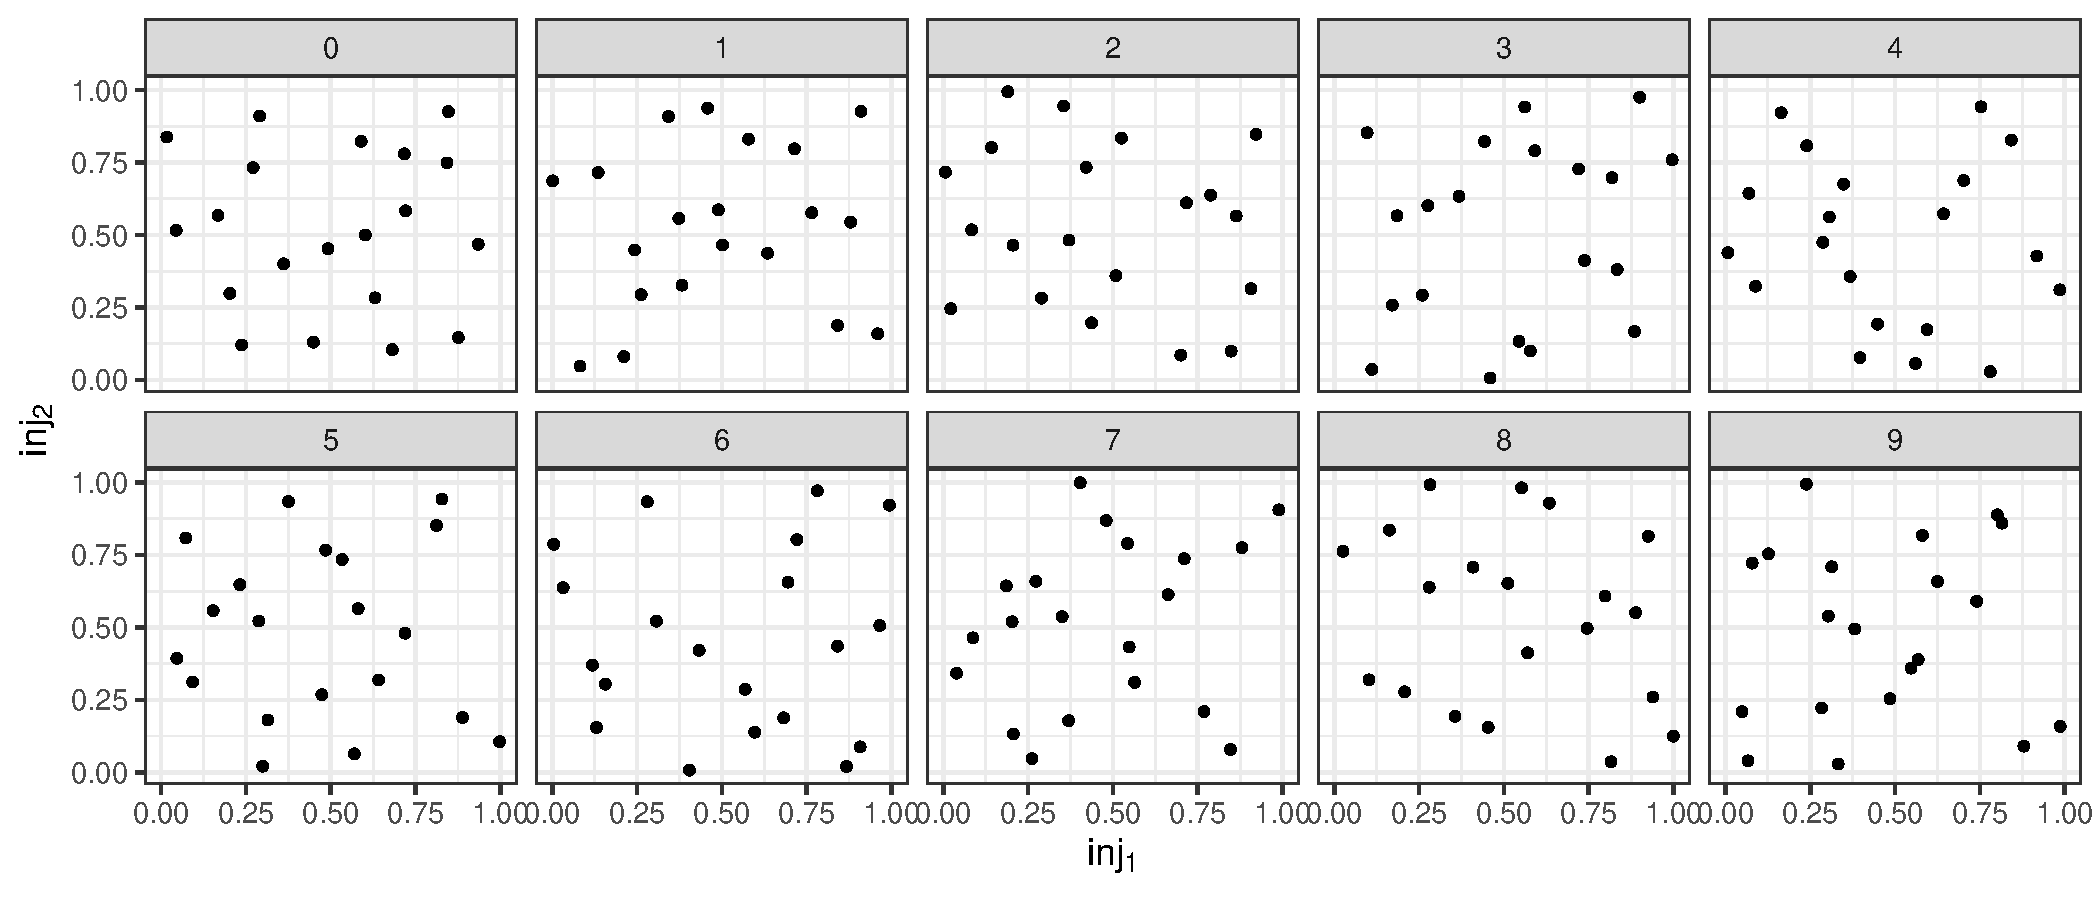
\includegraphics[width=0.8\textwidth]{./img/2_apps_min_mean_time/rs_20_samples_10_iterations_weighted_full_scatter.pdf}
\caption{\(inj_2\) in each of the 10 repetitions}
\end{figure}

\section{Histograms}
\label{sec:org12d167d}
Looking at the  histograms of the performance metric and  the execution times of
both  applications,  in  the  figure  below,  we see  that  almost  150  of  the
configurations tested had performance below \(10^{9}\).

\begin{center}
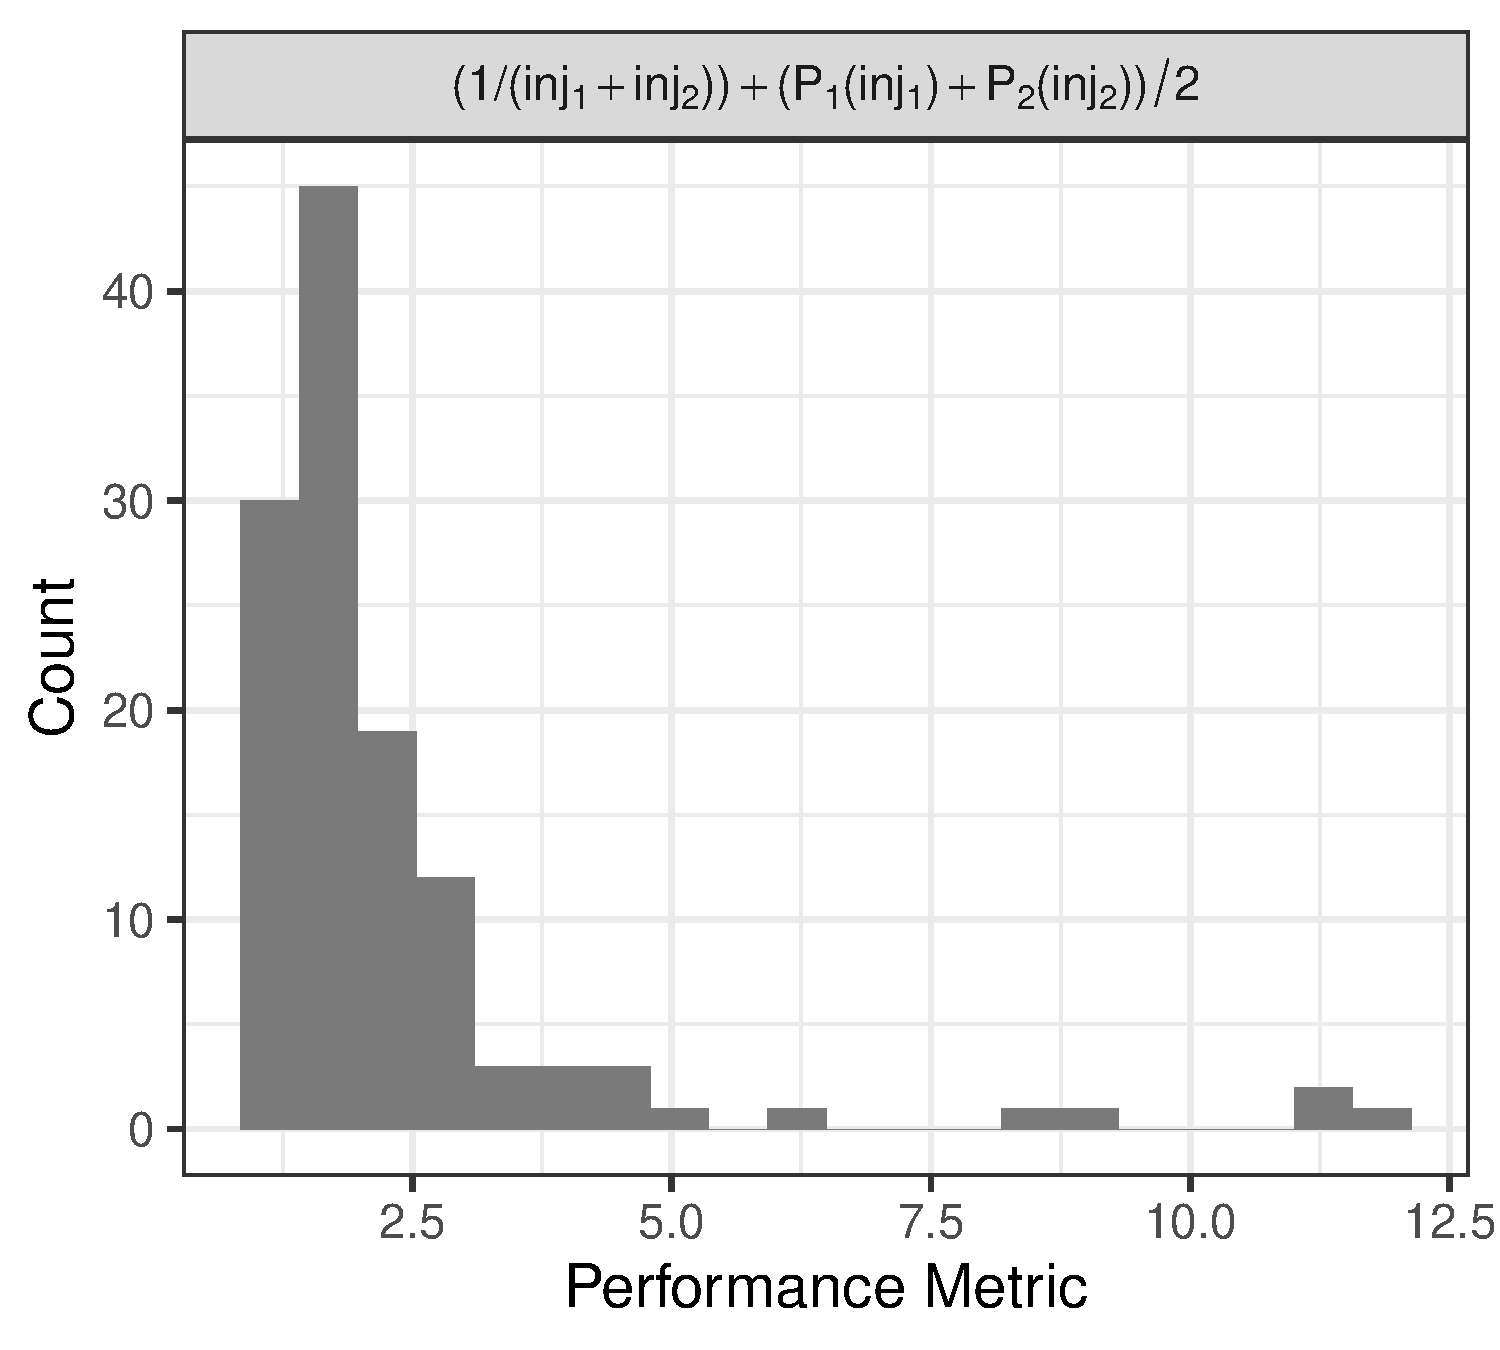
\includegraphics[width=0.5\textwidth]{./img/2_apps_min_mean_time/rs_20_samples_10_iterations_histogram_weighted_full.pdf}
\end{center}

\begin{center}
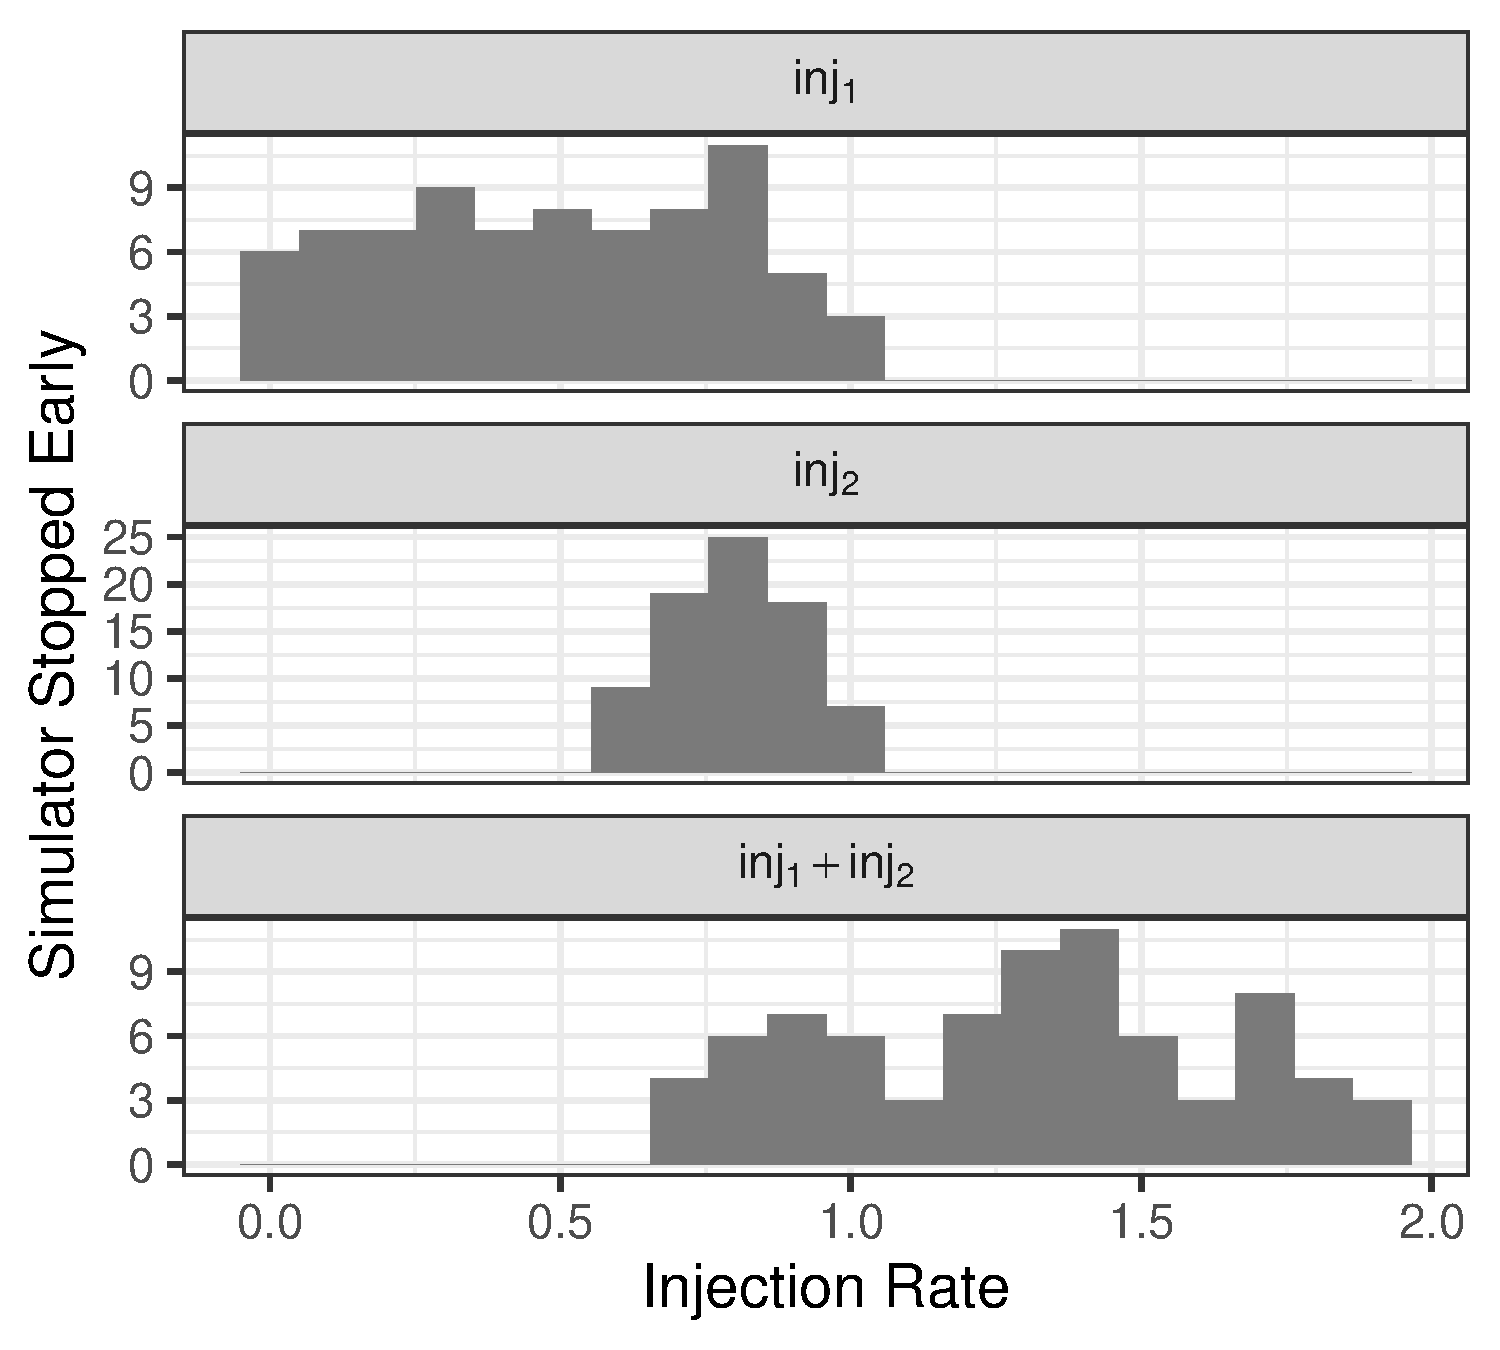
\includegraphics[width=0.5\textwidth]{./img/2_apps_min_mean_time/rs_20_samples_10_iterations_histogram_failed_weighted_full.pdf}
\end{center}

\begin{center}
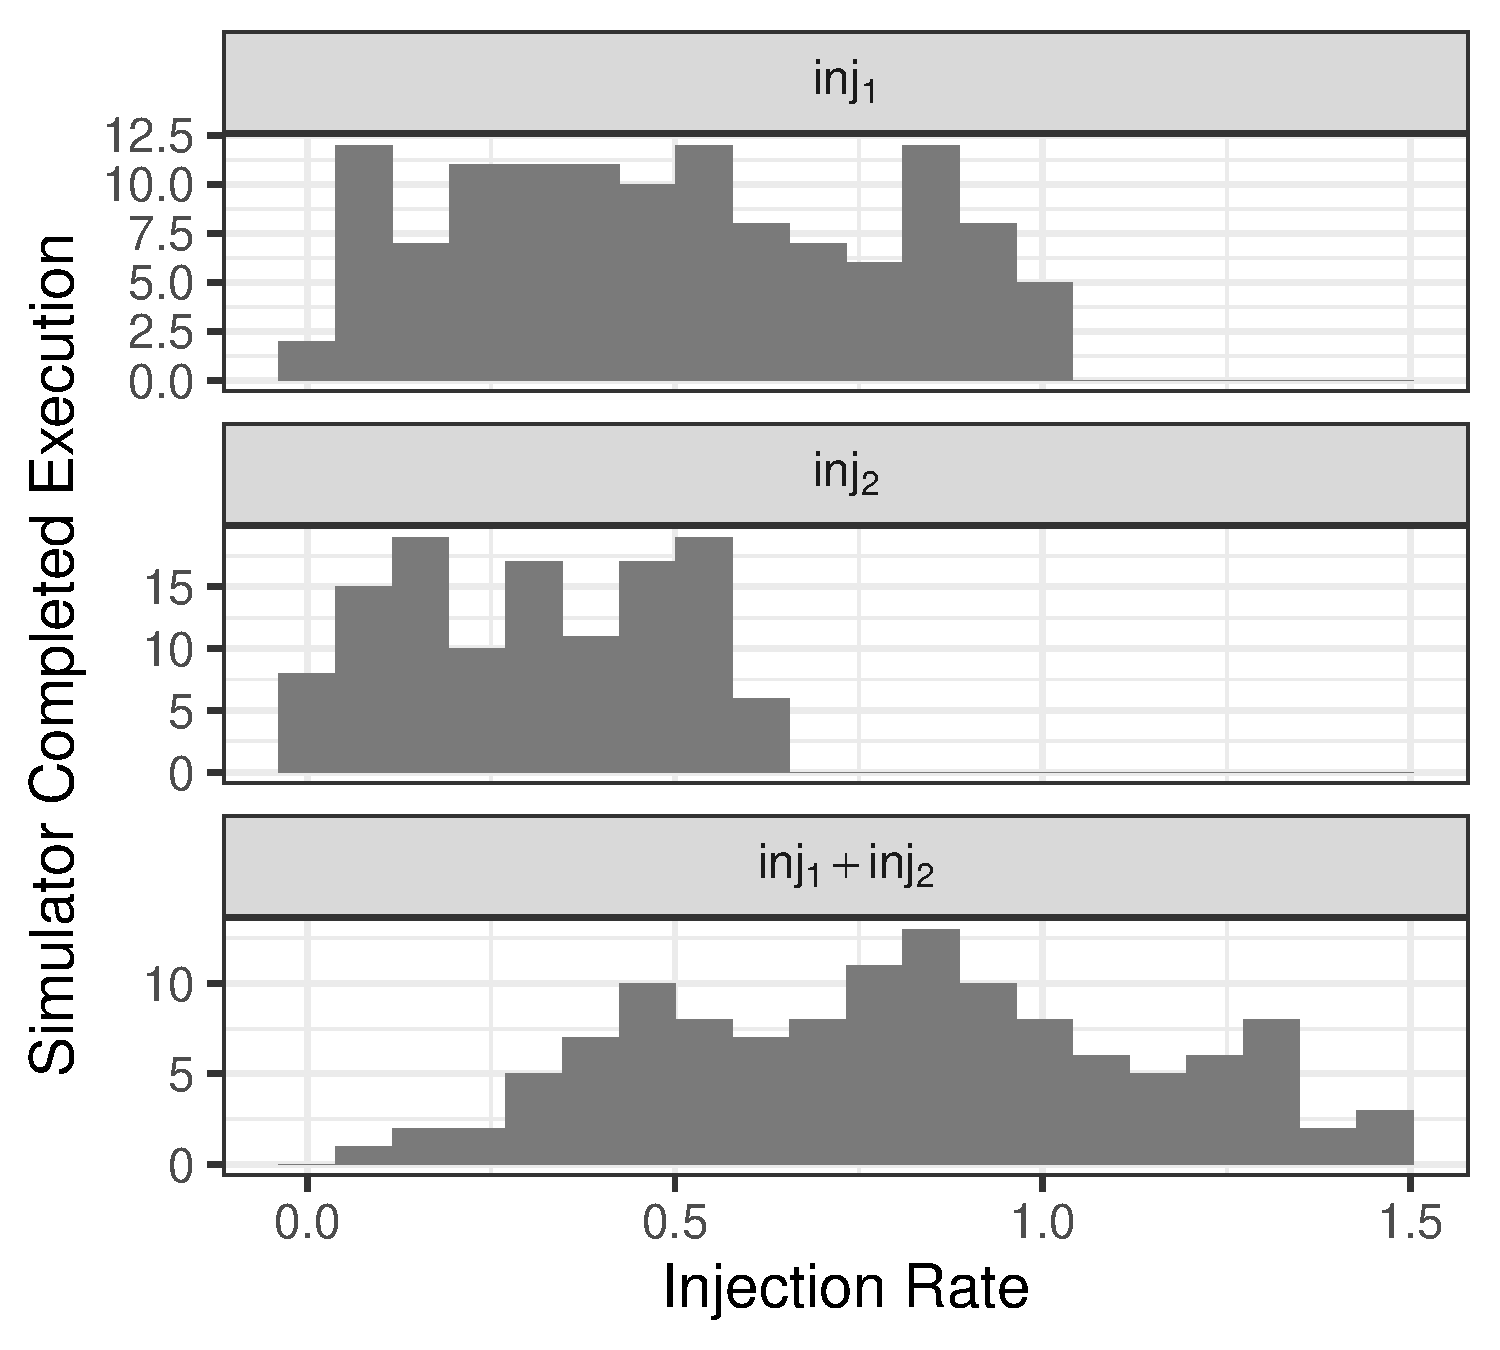
\includegraphics[width=0.5\textwidth]{./img/2_apps_min_mean_time/rs_20_samples_10_iterations_histogram_success_weighted_full.pdf}
\end{center}

\section{Mean Performance and Injection Rate}
\label{sec:orgc5d875d}
We  now  look  at  the  performance metric  measured  for  each  injection  rate
configuration.  The  figure below splits the  values of injection rate  for each
application, and shows the performance metric computed using the execution times
of both applications.

\begin{center}
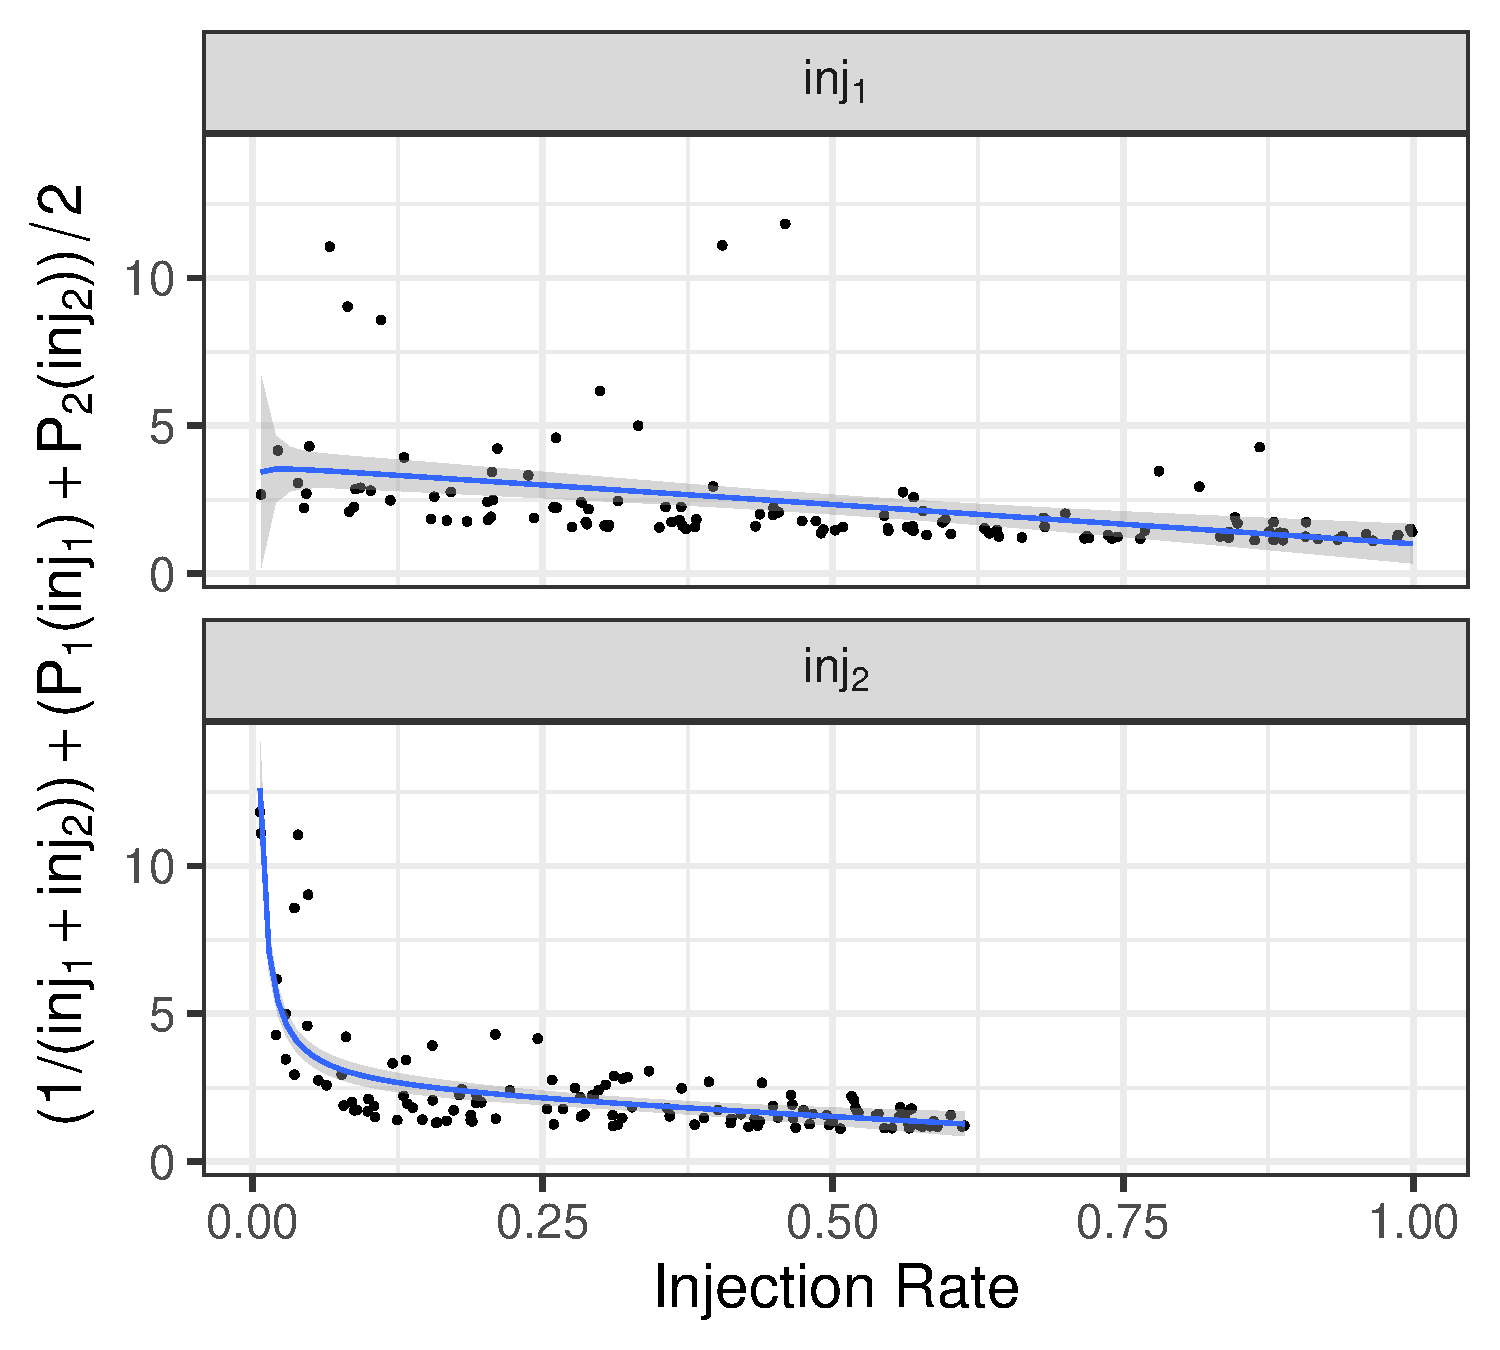
\includegraphics[width=0.6\textwidth]{./img/2_apps_min_mean_time/rs_20_samples_10_iterations_scatter_weighted_full.pdf}
\end{center}

\begin{center}
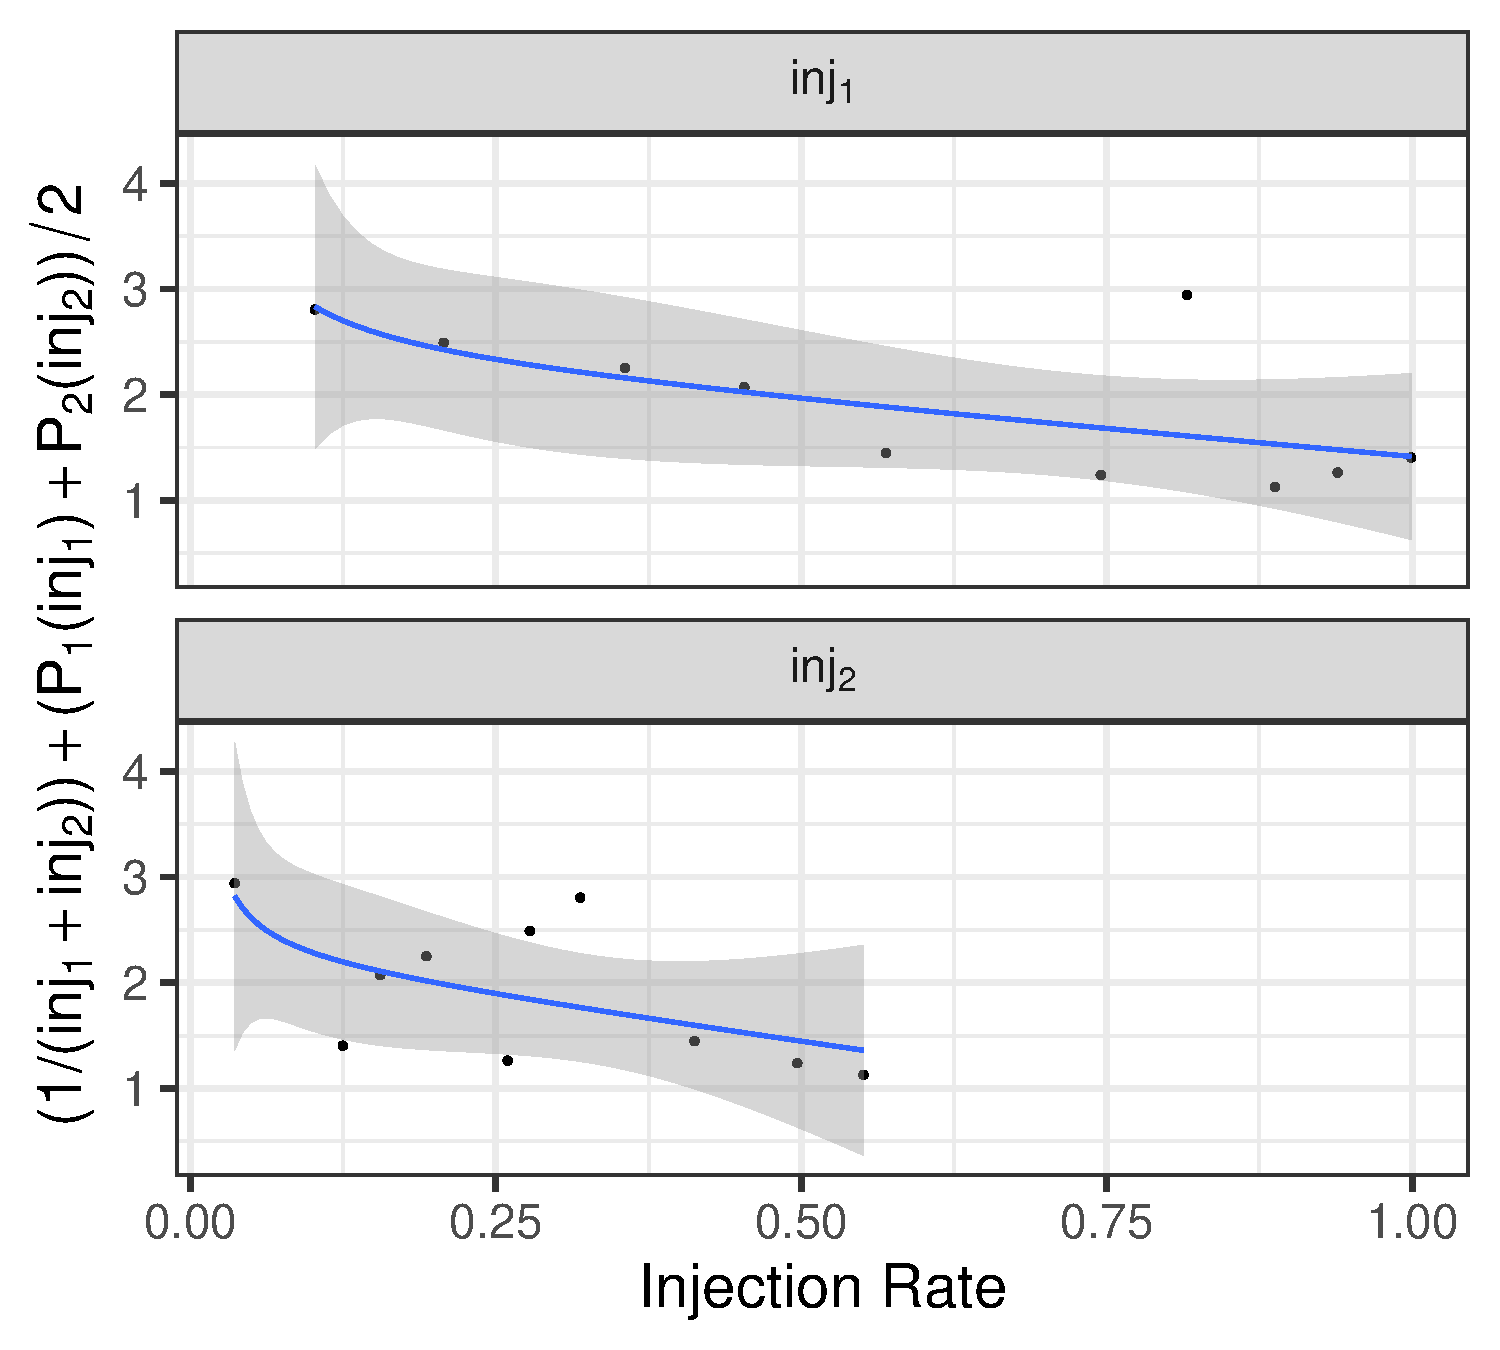
\includegraphics[width=0.6\textwidth]{./img/2_apps_min_mean_time/rs_20_samples_10_iterations_scatter_weighted_full_single.pdf}
\end{center}

The solid lines represent the fit of the collected data to the linear models
\begin{equation*}
\dfrac{\mathcal{P}(inj_1) + \mathcal{P}(inj_2)}{2} =
Y_1 = \beta_{1}inj_1 +
\beta_{2}\left(\dfrac{1}{inj_1}\right)\text{,}
\end{equation*}
for the top box, and
\begin{equation*}
\dfrac{\mathcal{P}(inj_1) + \mathcal{P}(inj_2)}{2} =
Y_2 = \beta_{3}inj_2 +
\beta_{4}\left(\dfrac{1}{inj_2}\right)\text{,}
\end{equation*}
for the bottom box. The shaded  regions represent the 95\% confidence interval of
the mean.

Visual inspection of  these fits indicates that \(inj_1\) does  not affect the mean
performance metric  as much as  \(inj_2\), which also have  a strong effect  in the
performance of application  1. The mean performance metric seems  to fit well to
the model using \(inj_2\).

\subsection{Scatters for other metrics}
\label{sec:org5031451}
\begin{center}
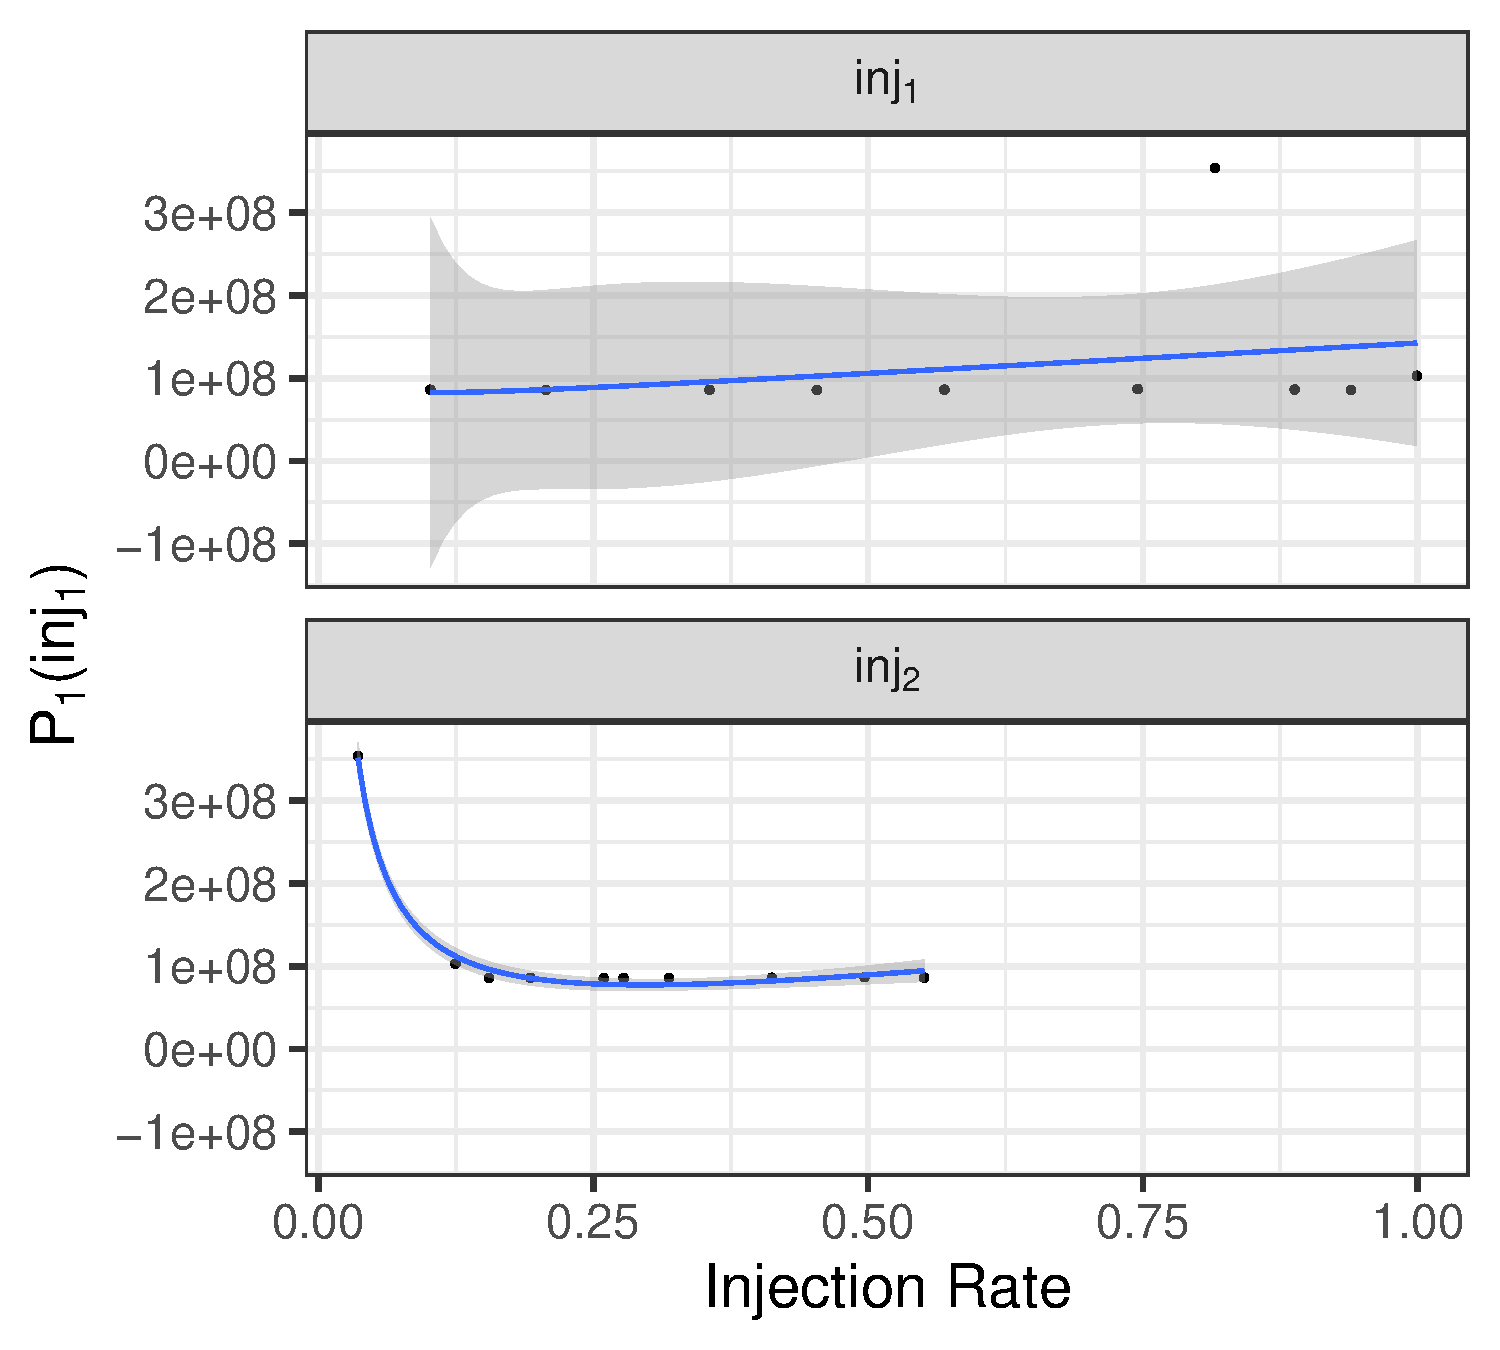
\includegraphics[width=0.6\textwidth]{./img/2_apps_min_mean_time/rs_20_samples_10_iterations_scatter_app1_weighted_full.pdf}
\end{center}

\begin{center}
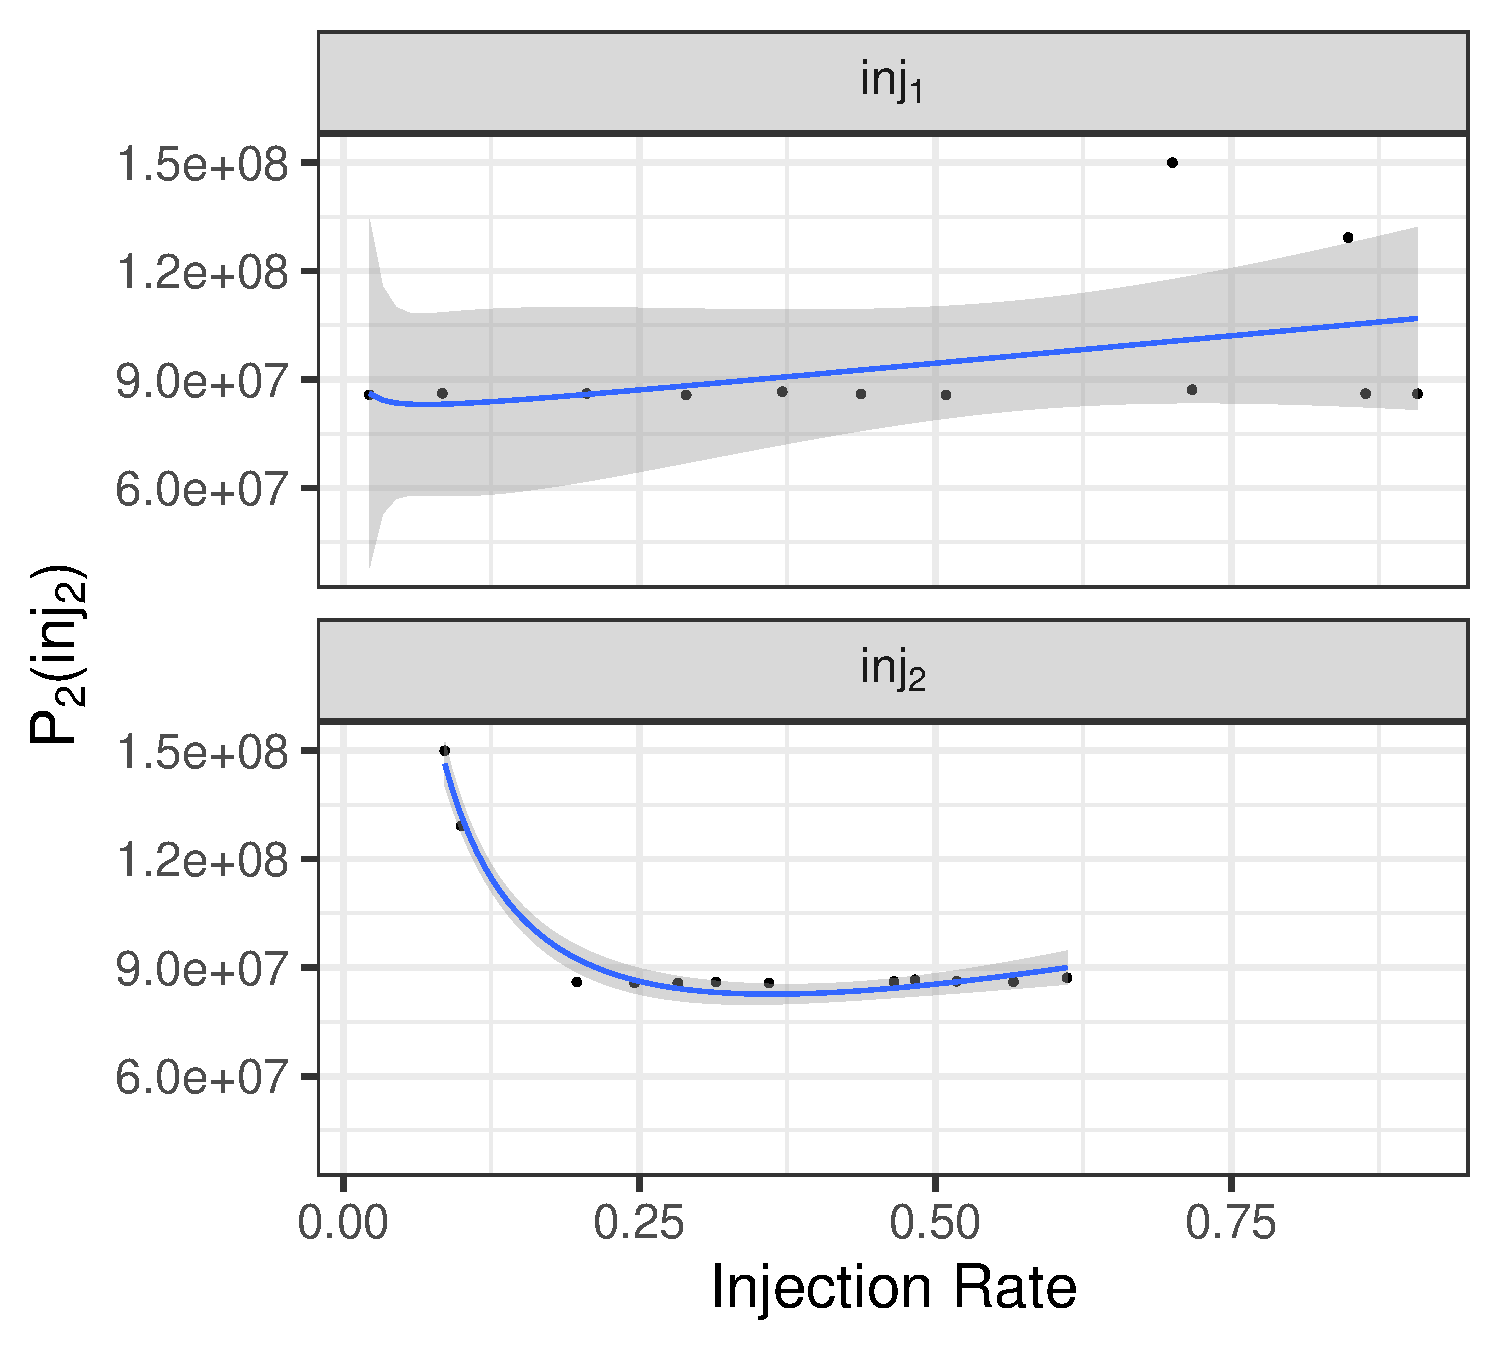
\includegraphics[width=0.6\textwidth]{./img/2_apps_min_mean_time/rs_20_samples_10_iterations_scatter_app2_weighted_full.pdf}
\end{center}

\section{ANOVA and Linear Model Fit}
\label{sec:orgd3fd749}
We  now perform  statistical  tests  to confirm  the  visual  analyses from  the
previous section.   We perform a  linear model fit using  the 20 samples  from a
single experiment, picked  at random between the 10  repetitions performed.  The
linear model we have used was
\begin{equation*}
\dfrac{\mathcal{P}(inj_1) + \mathcal{P}(inj_2)}{2} =
Y = \beta_{1}inj_1 +
\beta_{2}inj_2 +
\beta_{3}\left(\dfrac{1}{inj_1}\right) +
\beta_{4}\left(\dfrac{1}{inj_2}\right) +
\beta_{5}\left(inj_{1}inj_{2}\right) +
\beta_{6}\left(\dfrac{1}{inj_{1}inj_2}\right)\text{.}
\end{equation*}


% latex table generated in R 3.6.3 by xtable 1.8-4 package
% Thu Mar 12 11:52:03 2020
\begin{table}[ht]
\centering
\caption{Regression coefficients for a linear model fit using 20 experiments}
\begin{tabular}{lrr}
  \toprule
Model Term & Coefficient & Significance p-value \\
  \midrule
Intercept & $2.5 \times 10^{0}$ & $1.2 \times 10^{-4}$ \\
  injection\_rate\_1 & $-1.1 \times 10^{0}$ & $4.9 \times 10^{-2}$ \\
  injection\_rate\_2 & $-8.5 \times 10^{-1}$ & $2.2 \times 10^{-1}$ \\
  1/injection\_rate\_1 & $-1.0 \times 10^{-1}$ & $5.1 \times 10^{-3}$ \\
  1/injection\_rate\_2 & $-5.2 \times 10^{-2}$ & $1.6 \times 10^{-1}$ \\
  injection\_rate\_1 $\times$ injection\_rate\_2 & $2.6 \times 10^{-1}$ & $8.0 \times 10^{-1}$ \\
  1/injection\_rate\_1 $\times$ 1/injection\_rate\_2 & $6.0 \times 10^{-2}$ & $1.7 \times 10^{-3}$ \\
   \bottomrule
\end{tabular}
\end{table}

The  model coefficient  magnitude and  significance values  confirm that  \(inj_2\)
impacts the mean performance more than \(inj_1\), and the interaction between these
factors seem to not be significant  in this experiment. We also perform analysis
of variance,  using the same  performance mode,  for a single  20-run experiment
picked at random, shown in the table below.


% latex table generated in R 3.6.3 by xtable 1.8-4 package
% Thu Mar 12 11:52:38 2020
\begin{table}[ht]
\centering
\caption{Analisys of variance for a linear model fit using 20 experiments}
\begin{tabular}{lr}
  \toprule
Model Term & Significance p-value \\
  \midrule
injection\_rate\_1 & $1.5 \times 10^{-3}$ \\
  injection\_rate\_2 & $3.0 \times 10^{-5}$ \\
  1/injection\_rate\_1 & $6.9 \times 10^{-2}$ \\
  1/injection\_rate\_2 & $7.6 \times 10^{-4}$ \\
  injection\_rate\_1 $\times$ injection\_rate\_2 & $1.1 \times 10^{-1}$ \\
  1/injection\_rate\_1 $\times$ 1/injection\_rate\_2 & $1.5 \times 10^{-1}$ \\
  Residuals &  \\
   \bottomrule
\end{tabular}
\end{table}

We see again that  the terms using \(inj_2\) explain more  of the observed variance
on the performance metric. For further experiments using these two applications,
performance mean can be modeled and minimized using only a linear and an inverse
term  for  \(inj_2\).  Further  steps   should  be  attempting  to  generalize  the
statistical analysis  for more applications  running at  the same time,  or with
more controllable parameters.
\end{document}
